\documentclass{article}

% if you need to pass options to natbib, use, e.g.:
%     \PassOptionsToPackage{numbers, compress}{natbib}
% before loading neurips_2021

% ready for submission
\usepackage[preprint]{neurips_2021}

% to compile a preprint version, e.g., for submission to arXiv, add add the
% [preprint] option:
%     \usepackage[preprint]{neurips_2021}

% to compile a camera-ready version, add the [final] option, e.g.:
%     \usepackage[final]{neurips_2021}

% to avoid loading the natbib package, add option nonatbib:
%    \usepackage[nonatbib]{neurips_2021}

\usepackage[utf8]{inputenc} % allow utf-8 input
\usepackage[T1]{fontenc}    % use 8-bit T1 fonts
\usepackage{hyperref}       % hyperlinks
\usepackage{url}            % simple URL typesetting
\usepackage{booktabs}       % professional-quality tables
\usepackage{amsfonts}       % blackboard math symbols
\usepackage{nicefrac}       % compact symbols for 1/2, etc.
\usepackage{microtype}      % microtypography
\usepackage{xcolor}         % colors
\usepackage[pdftex]{graphicx}

\title{Analyzing Data of Accidents in France\\ from 2005 to 2016}

% The \author macro works with any number of authors. There are two commands
% used to separate the names and addresses of multiple authors: \And and \AND.
%
% Using \And between authors leaves it to LaTeX to determine where to break the
% lines. Using \AND forces a line break at that point. So, if LaTeX puts 3 of 4
% authors names on the first line, and the last on the second line, try using
% \AND instead of \And before the third author name.

\author{%
  Hannes Klein\\
  Matriculation No.: 5490178\\
 \texttt{hannes.klein@student.uni-tuebingen.de}\\
  \And
  Jonathan Reitemann\\
  Matriculation No.: 5729177 \\
  \texttt{jonathan.reitemann@student.uni-tuebingen.de}\\
  % examples of more authors
  % \And
  % Coauthor \\
  % Affiliation \\
  % Address \\
  % \texttt{email} \\
  % \AND
  % Coauthor \\
  % Affiliation \\
  % Address \\
  % \texttt{email} \\
  % \And
  % Coauthor \\
  % Affiliation \\
  % Address \\
  % \texttt{email} \\
  % \And
  % Coauthor \\
  % Affiliation \\
  % Address \\
  % \texttt{email} \\
}

\begin{document}

\maketitle

\begin{abstract}
  In this project for the course Data Literacy at the University of Tübingen, we analyzed a dataset of the \href{https://www.kaggle.com/ahmedlahlou/accidents-in-france-from-2005-to-2016?select=caracteristics.csv}{Accidents in France from 2005 to 2016}[1]. We are trying to analyze how the circumstances of these accidents affect the chances to lead to serious injuries and deaths. Therefore we first generate several simple plots and then use linear regression to see which of surrounding circumstances might be the most relevant to determine the severity of the injury. We put a special focus on comparing all accidents and accidents involving cyclists.
\end{abstract}

\section{Development over the years}

\iffalse
The first observation that is noticeable when looking at this dataset, is the number of people involved in accidents per year went down\ref{plot:severity1}. When we are looking at the severity of injuries we are also looking at a significant drop in all categories. The obvious question to ask is why the number of accidents went down and if we can find out with this dataset. For example the dataset tells us if an accident was near a bike lane but it doesn't tell us how many streets in France in total have bike lanes. 
\fi

The dataset contains the data of injuries in road and traffic accidents in France from 2005 until 2016. Looking at Figure \ref{plot:severity1} we can clearly see that the number of accident participants constantly decreases from 2005 until 2013 and then stagnates until 2016. When only looking at the bike accidents, the number seems to be relatively constant throughout the entire time period. There also is no major change in the percentage of severe injuries or deaths of people involved in accidents. This is both true when looking at all accidents and when only considering cyclists.\\

However, cyclists are clearly much less likely to come out of an accident unscathed. Both the percentages of light injuries and hospitalization is clearly much higher when only considering cyclists, compared to all people involved in accidents.

\begin{figure}
  \centering
  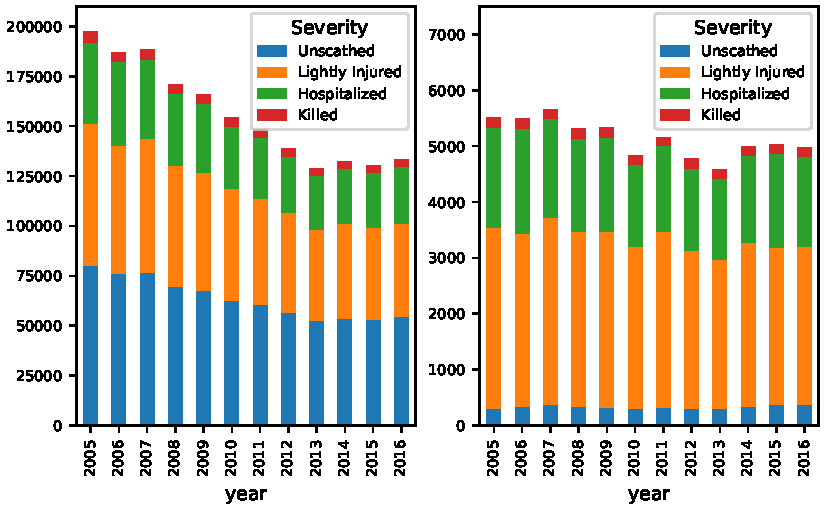
\includegraphics[]{Projekt/Plots/Accidents_per_year_and_severity.pdf}
  \caption{The number of people involved in accidents per year. The color shows their severity of injury.}
  \label{plot:severity1}
\end{figure}

\section{Effect of Road Categories}

We then decided to look at how much the severity of accidents varies between different road categories. Judging by Figure \ref{plot:severity_road} when considering all accidents, accidents on Department Roads and National Roads seem to have the highest death percentage, while highways seem to be somewhat safer. Department Roads especially stand out when considering the combined percentage of hospitalization and deaths. For cyclists, highways seem to have the highest death rate.
However, when considering the combined percentage of hospitalizations and deaths, national roads and department roads are by far the most dangerous.\\

It is however important to consider, that the sample size for highway accidents involving cyclists is 60, as they are generally not allowed to use them. 

\begin{figure}
  \centering
  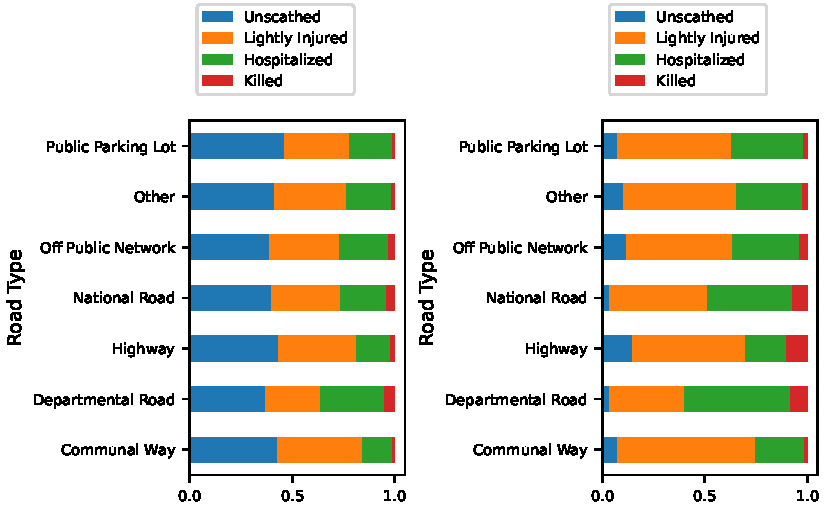
\includegraphics[]{Projekt/Plots/Comparison_of_percentages_of_severity_by_roadtype.pdf}
  \caption{The percentage of each severity by road category.}
  \label{plot:severity_road}
\end{figure}


\section{Predicting severity of accidents using Linear Regression}

In order to get a general idea of which circumstances of an accident increase the risk of severe injury, we used a linear regression model[2]. In order to be able to predict the level of injury with linear regression, we assigned an arbitrary value to each category:
Unscathed (0), Lightly Injured(10), Hospitalized(50) and Killed(100)

We applied linear regression twice: Once for considering all people involved in accidents, and once only considering cyclists.

\iffalse
With accidents we can look at the injuries that happen as an output. So if the severity of injuries is the output, the circumstances surrounding the accident is the input. With this thought we decided to use linear regression to predict the severity of injuries most likely caused by an accident.

\subsection{Input}

To predict the outcome of an accident we first have to ask which variables to consider. For example the name of the street is most likely not important as an explanatory variable. On the other hand we have illumination, weather condition, surface condition and road type, which probably are significant regarding the outcome. Then there are variables, like the reason for traveling or geographical coordinates, which are unclear in their significance.\\
We decided to keep most of the variables even if they most likely aren't relevant, since linear regression should identify them as irrelevant.

\subsection{Output}

On the other hand of linear regression is a scalar response which, in our case, is supposed to represent the most likely severity of injury. The dataset defines four levels of severity which are: 1: \textit{unscathed}, 2: \textit{killed}, 3: \textit{hospitalized wounded}, 4: \textit{light injury}. First we had to order these levels in terms of severity: 1: \textit{unscathed}, 2: \textit{light injury}, 3: \textit{hospitalized wounded}, 4: \textit{killed}.  But since this order does not seem to follow a linear fashion, we decided to change the indices to reflect this and use them as weights: 0: \textit{unscathed}, 10: \textit{light injury}, 50: \textit{hospitalized wounded}, 100: \textit{killed}. However, these weights are still almost arbitrary since it's impossible to put a specific value on human suffering.

\subsection{Linear Regression}

Using the specified input and output from our dataset we used linear regression to compute the coefficients shown in figure \ref{plot:regression1}. These coefficients can tell us the significance of their corresponding variable.

\begin{figure}
  \centering
  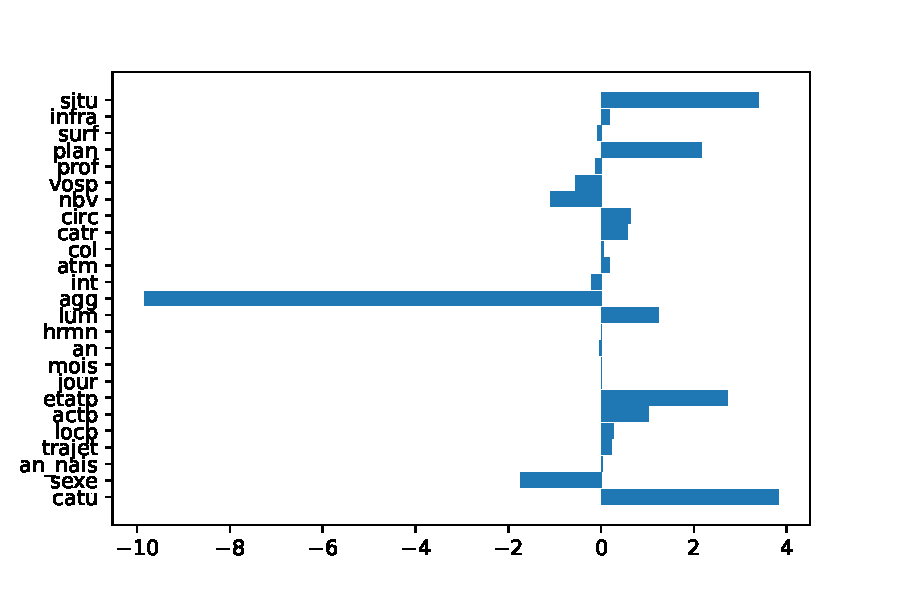
\includegraphics[width=1\linewidth]{Projekt/Plots/Linear_Regression_grav.pdf}
  \caption{The coefficients resulting from linear regression computed over all people.}
  \label{plot:regression1}
\end{figure}

\fi
\subsection{Explanatory Variables for Linear Regression}

The explanatory variables for our Linear regression model can be broadly separated into three categories:
\begin{itemize}
    \item Attributes of the person involved in the accident: This includes age, sex, participant category (which ranges from driver to pedestrian), numbers(which describes whether a pedestrian was alone or in a group, when applicable) action (whether the pedestrian was on the sidewalk or crossing the road) and location(describes location of pedestrian, including distance from traffic lights and whether he/she was on a sidewalk, road or traffic aisle) 
    \item Attributes of the road section: This includes curvature and gradient of the road, road type(from parking lot to highway), infrastructure(in a tunnel, on a bridge, railway), number of lanes, traffic regime(one-way, bidirectional, separated carriageways) or agglomeration(whether the accident happened inside or outside an agglomeration), bikepath(existence of a bikepath)
    \item Attributes of general conditions: Weather, Surface conditions, collision type, lighting(from daylight to public lighting to Night), time of day, year, month and day of the accident
\end{itemize}
\iffalse
The following variables were used as the explanatory variables for or linear regression model:

\begin{itemize}
    \item Accident Location:\\
    This variable describes the location of the accident on the road. It can take values from 1 - 5 increasing from 'on the road' via 'on the emergency stop band' towards 'on the bikepath/sidewalk'
    \item Infrastructure:\\
    This variable describes whether the accident happened on some kind of special infrastructure, for e.g. in a tunnel, on a bridge or in a pedestrian zone. 
    \item Surface condition:\\
    Whether there where any special road conditions, like a wet, icy, muddy or snowy surface
    \item Road Curvature:
    Describes if the accident happened in a straight, left/right curved or s-curved road section.
    \item Road Gradient
    \item Bikepath:\\
    Describes whether a bikepath exists at the accident location. Differentiates between bikepaths, Cycle Banks and Reserved Channels.
    \item Number of lanes:\\
    Number of traffic lanes at the accident location
    \item Traffic regime:\\
    Ascending from One-way via bidirectional towards separated carriageways on highways
    \item Collision Type: \\
    Describes the type of collsion (frontal/from the rear) and the number of vehicles involved.
    \item Weather
    \item Intersection:\\
    Describes if the accident happened at an interception and the type of intersection, for e.g. X/T/Y-intersections
    \item Agglomeration:\\
    Whether or not the accident happened within or outside an agglomeration
    \item Year/month/day
    \item Number/Action/Location of pedestrian:\\
    Variables to describe whether pedestrians involved in the accident where alone, crossing the road or standing on the sidewalk, and whether they were on the sidewalk, bikepath or the road when the accident happened. 
    \item Age
    \item Sex
    \item Participant category:\\
    Driver, Pedestrian or Passenger

\end{itemize}
\fi
\iffalse
\subsubsection{Accident Location}

This variables tells us the traffic lane the accident took place. It has the following possible values: 1: \textit{On The road}, 2: \textit{On emergency stop band}, 3: \textit{On the verge}, 4: \textit{On the sidewalk}, 5: \textit{On bike path}. Although this order is arbitrary the coefficient puts a high importance on it. That is possibly because the highest value concerns bike paths. Accidents on bike paths most likely involve cyclists and cyclist have a high risk of injury, due to less protection than someone in a car.

%\subsubsection{Infrastructure}

%This variable shows different type of infrastructure, like tunnels, bridges or railways. The coefficient shows a small significance.
%Der Wert hat in 89% der Fälle eine 0(keine spezielle infrastructure)

%\subsubsection{Surface Condition}

%Surface conditions seem to have a very low impact on severity of injuries. To understand why we have to look at the specific values and their meaning: 1: \textit{normal}, 2: \textit{wet}, 3: \textit{puddles}, 4: \textit{flooded}, 5: \textit{snow}, 6: \textit{mud}, 7: \textit{icy}, 8: \textit{fat/oil}, 9: \textit{other}. Unfortunately This order is almost arbitrary. For example it is unclear if a flooded road is more difficult to drive on than a road with snow on it. If the list does not follow a strict order of severity, it is hard for linear regression to put a coefficient on the variable.

\subsubsection{Road curvature}

This variable shows the shape of the road: 1: \textit{straight part}, 2: \textit{curved left}, 3: \textit{curved right}, 4: \textit{form of an "S"}. There is a relatively high coefficient on it, since the form of an "S" has the highest index and is probably the most difficult to drive.

%\subsubsection{Road gradient}

%This variable shows the shape of the road in profile: 1: \textit{dish}, 2: \textit{slope}, 3: \textit{hilltop}, 4: \textit{hill bottom}. The coefficient shows a low significance for this variable.

%\subsubsection{Bike path}

%This variable shows the existence of a bike path or something similar on the road of the accident: 1: \textit{bike path}, 2: \textit{cycle bank}, 3: \textit{reserved channel}. 
%It should be noted that we are unclear about what a cycle bank exactly is.
%The coefficient shows a small negative impact on severity, which shows that a reserved lane for cyclists is at least slightly beneficial.

\subsubsection{Number of lanes}

The coefficient for this variable shows small negative impact, which means that more lanes increase the severity of injuries.

%\subsubsection{Traffice regime}

%This variable has the following possible values: 1: \textit{one way}, 2: \textit{bidirectional}, 3: \textit{separated carriageways}, 4: \textit{with variable assignment channels}. The coefficient is slightly positive which could be because the indices show kind of a rising level of complexity which probably makes the road more dangerous.

%\subsubsection{Road type}

%\subsubsection{Collision type}

%\subsubsection{Weather}

%\subsubsection{Intersection}

\subsubsection{Agglomeration}

\subsubsection{Lighting}

%\subsubsection{Time of day}

%\subsubsection{Year}

%\subsubsection{Month}

%\subsubsection{Day}

\subsubsection{Number of pedestrians}

\subsubsection{Action of pedestrian}

%\subsubsection{Location of pedestrian}

%\subsubsection{Travel reason}

%\subsubsection{Age}

\subsubsection{Sex}

\subsubsection{Participant category}

\subsection{Linear regression on only cyclists}

\begin{figure}
  \centering
  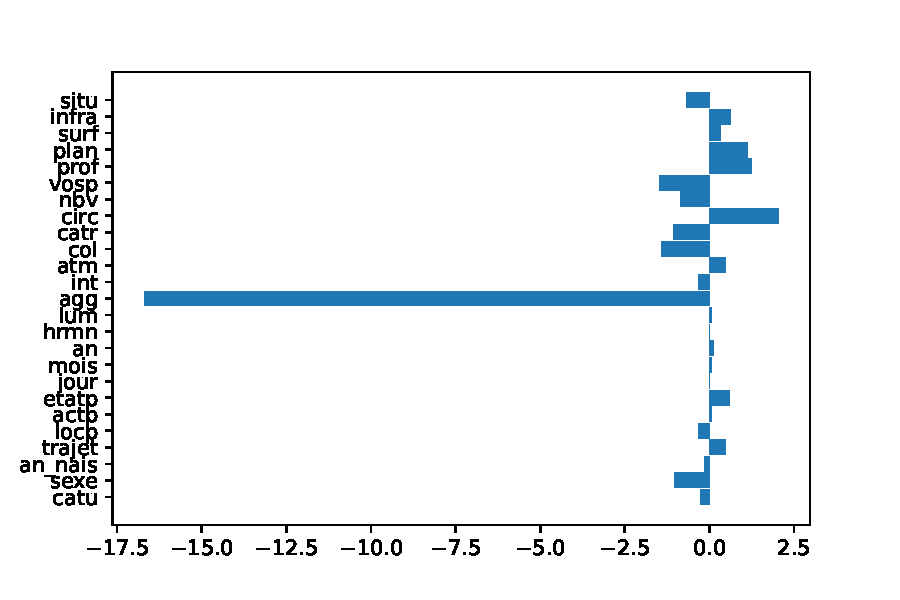
\includegraphics[width=1\linewidth]{Projekt/Plots/Bike_Linear_Regression_grav.pdf}
  \caption{The coefficients resulting from linear regression computed over all cyclists.}
  \label{plot:regression2}
\end{figure}

\subsection{Problems with linear regression}

The first problem with linear regression on this problem is that explanatory variables might not have a logical order. For example surface conditions are ordered the following way in this dataset: 1: \textit{normal}, 2: \textit{wet}, 3: \textit{puddles}, 4: \textit{flooded}, 5: \textit{snow}, 6: \textit{mud}, 7: \textit{icy}, 8: \textit{fat/oil}, 9: \textit{other}.
However, this order is almost completely arbitrary. For example it is unclear if a flooded road is more difficult to drive on than a road with snow on it. So if the list does not follow a strict order of severity, it is hard for linear regression to put a coefficient on that variable.\\
A similar problem occurs with predictions over the time of the day. Although the time of day at least has a strict sequential order, the significance is most likely not along this order. For example we can imagine that during rush hours, which occur in the morning and in the evening, would probably be a noticeable rise of accidents. But linear regression can only put importance on either high or low numbers, so it can't identify specific time slots.
\fi

\subsection{Results of Linear Regression}

\begin{figure}
  \centering
  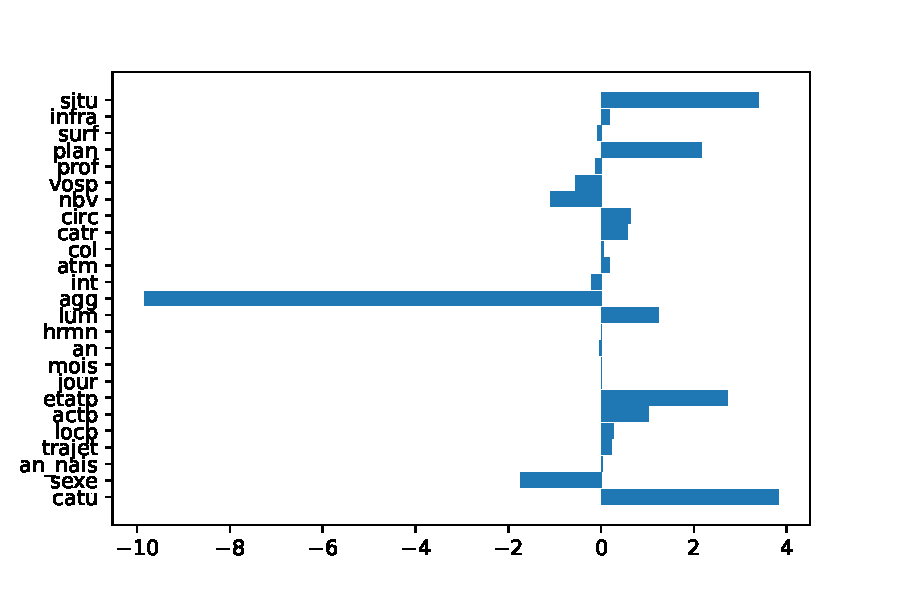
\includegraphics[]{Projekt/Plots/Linear_Regression_grav.pdf}
  \caption{The coefficients resulting from linear regression computed over all participants.}
  \label{plot:regression_all}
\end{figure}

\begin{figure}
  \centering
  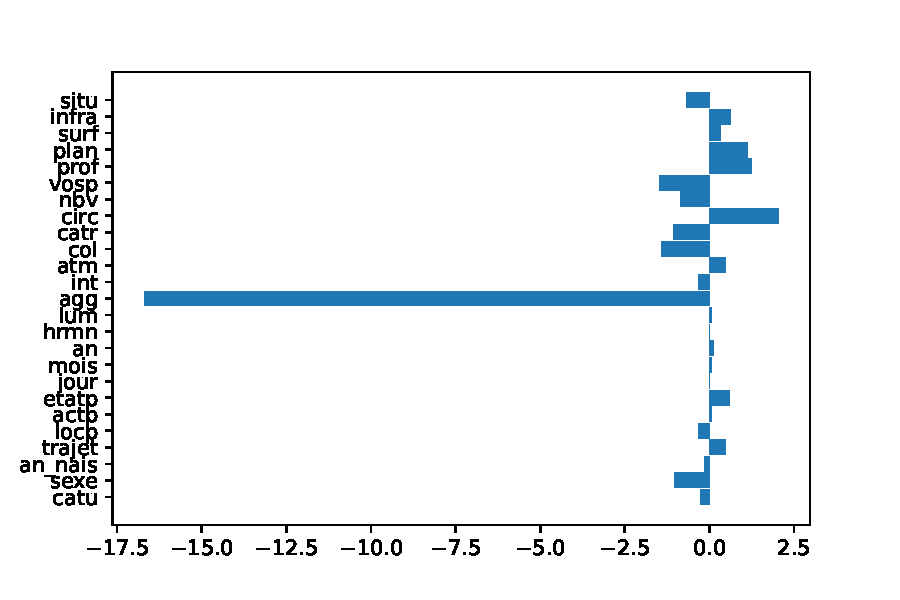
\includegraphics[]{Projekt/Plots/Bike_Linear_Regression_grav.pdf}
  \caption{The coefficients resulting from linear regression computed over all cyclists.}
  \label{plot:regression_bikes}
\end{figure}

Figure \ref{plot:regression_all} shows the coefficient of each explanatory variable when predicting the injury severity of all accident participants while Figure \ref{plot:regression_bikes} shows the coefficients when only considering cyclists. Whether or not an accident happened inside or outside of an agglomeration seems to be by far the most important factor in both cases, with injuries being much more severe in accidents outside of agglomerations. Other very relevant factors seem to be road curvature and gradient, the number of lanes and the participant category. According to our linear regression model, the time of day, year, date, surface condition, weather and Location of pedestrians seem to be nearly completely irrelevant.

\subsection{Criticisms of Linear Regression on this dataset}

Some of the results of our linear regression model seem somewhat surprising. While it is somewhat reasonable that accidents outside of agglomerations are more dangerous than those within agglomerations, it seems unlikely that this should be the most important factor by that margin. Some other variables seem surprisingly irrelevant: This includes weather conditions, surface conditions, month and time of day.\\

This can be explained by the fact, that many of the variables may not be linear factors. As an example, when considering time of day, conditions do not change in a linear fashion from 0 am to 12 pm. The same applies to months: Conditions are very similar in January and December, while these are the two most extreme points in our numerical representation. For other variables, like action or location of pedestrians, collision types, intersection type or participant category, weather or surface conditions, it is difficult or impossible to find an objective ordering of possible values. It seems impossible to put the categories muddy, snowy, wet, icy and oily/fat in an objective linear order, which leads to those being evaluated somewhat arbitrarily by linear regression. This might also be the reason, why linear regression considers categories like agglomeration or road gradient to be so important. These categories likely have an effect on severity of injury, and can be easily ordered.

\medskip
\section*{References}
{
\small
[1] Accidents in France from 2006 to 2016,
Owner: Ahmed Lahlou Mimi,
URL:https://www.kaggle.com/ahmedlahlou/accidents-in-france-from-2005-to-2016,
License: CC0: Public Domain

[2] Link to our repository: https://github.com/whyisnousernameavailable/Data\_Literacy\_project
}

\end{document}
